\documentclass[twocolumn]{article}
\usepackage{geometry}
\geometry{a4paper, top=2.5cm, left=2cm, right=2cm, bottom=2.5cm}
\usepackage{graphicx}
\usepackage{subcaption}
\usepackage{tikz}
\usetikzlibrary{positioning,fit,shapes.geometric,backgrounds}
\usepackage{hyperref}
\usepackage{amsmath}
\usepackage{amssymb}
\usepackage{authblk}
\renewcommand*{\Authand}{ و }
\renewcommand*{\Authands}{ و }
\usepackage{xepersian}
\settextfont{XB Niloofar}
\newcommand{\mykeyword}[1]{\par\textbf{واژه‌های کلیدی:}{#1}}
%%%%%%%%%%%%%%%%%%%%%%%%%%%%%
%%%%%%%%%%%%%%%%%%%%%%%%%%%%%%%
\begin{document}
\title{احتمال تعمیم‌پذیر نبودن روش‌های ارزیابی کیفیت مبتنی بر بردار پشتیبان}
% \author{آرمین احمدزاده \thanks{a.ahmadzadeh@ipm.ir}}
% \author{پوریا چراغی \thanks{cheraaqee@ipm.ir}}

\author[1]{آرمین احمدزاده \thanks{a.ahmadzadeh@ipm.ir}}
\author[2]{پوریا چراغی \thanks{cheraaqee@ipm.ir}}
\author[3]{حمید سربازی آزاد \thanks{azad@sharif.edu} \thanks{azad@ipm.ir}}
% % \author[3]{حسین معتمدنیا \thanks{h.motamednia@ipm.ir}}
% \author[3]{محمد مینویی \thanks{mohammad.minouei@dfki.de}}
% \author[4]{آزاده منصوری \thanks{a\_mansouri@khu.ac.ir}}
% \author[5]{احمد محمودی ازناوه \thanks{a\_mahmoudi@sbu.ac.ir}}
\affil[1,2,3]{مرکز پردازش سریع، پژوهشکده علوم کامپیوتر، پژوهشگاه دانش‌های بنیادی، تهران، ایران}
\affil[3]{دانشکده مهندسی کامپیوتر، دانشگاه صنعتی شریف، تهران، ایران}
% \affil[3]{گروه علوم کامپیوتر، دانشگاه صنعتی کایزرسلاترن، کایزرسلاترن، آلمان}
% \affil[4]{گروه مهندسی برق و کامپیوتر، دانشکده فنی، دانشگاه خوارزمی، تهران، ایران}
% \affil[5]{پژوهشکده مطالعات سایبری، دانشگاه شهید بهشتی، تهران، ایران}
\date{}

\maketitle
\begin{abstract}
	یک مدل محاسباتی که بتواند نظرِ انسان در موردِ کیفیتِ تصاویر را پیش‌بینی نماید، کاربردهای فراوانی در مسائل مربوط به پردازش تصویر دارد. به دلیلِ پیچیدگی دستگاه بینایی بشر، مدل‌های یادگیری ماشین برای شبیه‌سازیِ نحوه‌ی قضاوتِ انسان‌ها استفاده می‌شوند. یکی از این مدل‌ها، وایازش بردار پشتیبان است. در این مقاله، نشان می‌دهیم که روش رایج برای بکارگیریِ بردارِ پشتیبان در ارزیابی کیفیت تصویر، لزوماً به مدل‌های قابل ِ تعمیم نمی‌انجامد.
\end{abstract}
% \begin{keyword}
\mykeyword{هوش مصنوعی، پردازش تصویر، دستگاه بینایی انسان، یادگیری ماشین، ارزیابی کیفیت تصویر، نمامفاد، ماشین بردار پشتیبان، وایازش }
% \end{keyword}




\section{مقدمه}
\label{sec:intro}
تصاویر دیجیتال بخش قابل توجهی از مصرف رسانه‌ای بشر را تشکیل می‌دهند \cite{cisco}. بدیهی است که کیفیّتِ کَمِ این رسانه، منجر به نارضایتی کاربران و ناکامی ما در دریافت اطّلاعات مدّنظرمان خواهد شد. لذا، مطلوب است که وضعیت تصاویر ارسالی، از منظر کیفیت‌شان، تحت نظارت باشد.

مطمئن‌ترین راه برای ارزیابی کیفیت تصویر (که به اختصار «اَکْتْ» می‌خوانیمش)، پرسش از انسان‌هاست \cite{allen2012manual}. به این ترتیب که تصویری را به جمعی از ناظرین\RTLfootnote{همان «\lr{subject}»ها در آزمایش‌های علمی} نشان داده و نظر آن‌ها در مورد کیفیت تصویر را در قالب نمره‌ای از یک بازه‌ی مشخّص (، مثلاً $[0, 100]$،) جویا می‌شویم. میانگین نظرات\RTLfootnote{که به اختصار «\lr{MOS}» نامیده می‌شود و مخفّف عبارت «\lr{Mean Opinion Score}» است. لازم به توضیح است که «\lr{MOS}» نسبت مستقیمی با کیفیت ادراکی و «\lr{Difference-MOS}» یا «\lr{DMOS}» نسبتی عکس با کیفیت تصویر دارد.}، یک کمّیّت قابل اطمینان از کیفیّت تصویر است \cite{mohammadi2014subjective}. چنین آزمایشی نیز اَکْتِ «انسانی\LTRfootnote{subjective image quality assessment}» نام دارد.

بدیهی است که اَکْتِ انسانی برای کاربردهای بر-خط\RTLfootnote{معادل فارسی «\lr{on-line}»} و حجیم امکان‌پذیر نیست. در این موارد، نرم‌افزاری مطلوب است که بتواند قضاوت دستگاه بینایی بشر در مورد کیفیت یک تصویر را پیش‌بینی نماید. دقت و سرعت این پیش‌بینی، معیارهای عملکرد یک مدل محاسباتیِ اَکْتْ\LTRfootnote{objective image quality assessment} هستند. ساخت چنین مدلی، موضوع مورد مطالعه‌ی بخش قابل توجهی از تحقیقاتِ پردازش تصویر است\cite{zhai2020perceptual}. برای ارزیابی و آموزش روش‌های محاسباتی، از نتایج اَکْتِ انسانی استفاده می‌شود.

ساده‌ترین راه برای اَکْتِ محاسباتی، محاسبه‌ی اختلاف دو تصویر است. موارد زیادی وجود دارند که یک تصویر سالم (با کیفیت احتمالاً مطلوب،) دچار تخریب شده و یک نسخه‌ی تخریب‌شده از آن بوجود می‌آید. وقتی هردوی این دو تصویر در دسترس باشند، می‌توان برای ارزیابی کیفیِت تصویرِ تخریب‌شده، به اطلاعات موجود در تصویر سالم رجوع کرد. به این کار اَکْتِ «مرجع کامل» گفته می‌شود \cite{larson2010most}. یک مثال از کاربرد اَکْتِ مرجع کامل، فشرده‌سازی تصاویر است. الگوریتم فشرده‌کننده با کاهش اطلاعاتِ نشانک\RTLfootnote{معادل فارسی «\lr{signal}»}، حجم آن را کاهش داده و از طرفی کیفیّت آن را نیز خدشه‌دار می‌نماید. الگوریتم اَکْتِ مرجع کامل می‌تواند در هر لحظه تصویر فشرده‌شده را با تصویر اصلی مقایسه کرده و در صورت تخریبِ بیش از حدِّ کیفیت، این مورد را به الگوریتم فشرده‌کننده بازخورد دهد \cite{eckert1998perceptual}.

اگر $x(i, j)$ نشانک مرجع و $y(i, j)$، نشانک تخریب‌شده باشد، میانگین مربّعات خطا، «\lr{MSE}\LTRfootnote{Mean Squared Error}»، اختلاف مقادیر آن دو را خواهد سنجید:
\begin{equation}
	MSE(x, y) = \displaystyle \frac{1}{M\times N} \sum_{i=1}^M\sum_{j=1}^N (x(i, j)- y(i, j))^2
\label{eq:mse}
\end{equation}
$M$ و $N$ در~(\ref{eq:mse})، ابعاد تصاویر هستند. 
نشان داده می‌شود که «\lr{MSE}» یا بیشینه‌ی نسبت نشانک به نوفه\RTLfootnote{معادل فارسی «\lr{noise}»}، «\lr{PSNR}\LTRfootnote{Peak Signal-to-Noise Ratio}»، نمی‌توانند درک انسان از کیفیت تصویر را شبیه‌سازی نمایند \cite{wang2009mean}. وانْگْ\LTRfootnote{Zhou Wang} و همکارانش نشان دادند که تخریب ساختارهای تصویر در کاهش کیفیت آن مؤثر است\cite{wang2009mean}. در سال ۲۰۰۴، روشی به نام «\lr{SSIM}\LTRfootnote{Structural Similarity}» برای کمّی‌سازی شباهت ساختاری دو تصویر ارائه کردند \cite{wang2004image} که با اختلاف از روش‌های مبتنی بر-«MSE» بهتر بود \cite{sheikh2006statistical}.  

با موفقیتِ \lr{SSIM}، محققین سعی کردند ساختارهای تصویر را با ویژگی‌های دیگری، مثل لبه‌ها، مدل کنند. آماره‌های تصاویر طبیعی\LTRfootnote{\lr{Natural Scene Statistics- NSS}} \cite{ruderman1994statistics} و پایداری اطلاعاتی\LTRfootnote{\lr{Information Fidelity}} \cite{sheikh2006image}، دیگر معیارهای پیشنهاد شده برای کیفیت تصویر هستند. روش‌های یادگیری ماشین سر-تا-سری\LTRfootnote{\lr{end-to-end}} نیز، برای اَکْتِ محاسباتی استفاده شده‌اند \cite{kim2017deep, yang2019survey, ye2012unsupervised}.

یک ساز و کار رایج برای اَکْتْ، استفاده از ماشین بردار پشتیبان، «\lr{SVR}\LTRfootnote{Support Vector Regression}» \cite{vapnik1999nature} است \cite{cheraaqee}. کلّیات بکارگیری «SVR» در شکل~\ref{fig:svr} دیده می‌شود.
\begin{figure}
	\begin{center}
		\begin{tikzpicture}
			\begin{scope}[scale=0.8, transform shape]
			% \draw[step=1cm, gray, very thin] (0, -5) grid (15, 4);
				\draw[thick] (0,0)--(0,2.5)--(1.5,3.5)--(1.5,1)--(0,0);
				\node[rotate=90] at (0.75,1.5) {\hboxR{تصویر ورودی}};
				\draw[dashed, thick] (0,-3.5)--(0,-1)--(1.5,0)--(1.5,-2.5)--(0,-3.5);
				\node[rotate=90] at (0.75,-2) {\hboxR{تصویر مرجع}};
				\draw[blue, ->] (1.5, 3) -- (3.5, 3);
				\draw[blue, dashed] (1.5, -0.5) -- (2.7, -0.5) -- (2.7, 2.5);
				\draw[blue, dashed, ->] (2.7, 2.5) -- (3.5, 2.5);
				\node[fill=blue!20] (feactorator) at (5, 2.7) {\hboxR{استخراج‌کننده‌ی ویژگی}};
				\node[draw] (feactor) at (8.4, 2.7) {\hboxR{بردار ویژگی ($\vec{f}_{1\times F}$)}};
				\draw[->] (feactorator.east) -- (feactor.west);
				% \draw[blue] (8.4, 2.3) -- (8.4, 1.7);
				% \draw[blue, ->] (8.4, 1.7) -- (7.8, 1.7);
				\node[fill=blue!20] (svr) at (5.9, 1.5) {\hboxR{«\lr{SVR}» ِ آموزش‌دیده}};
				\draw[blue, ->] (feactor.south) |- (svr.east);
				\node[draw] (qscore) at (5.9, -0.3) {\hboxR{تخمینِ زده‌شده از نمره‌ی کیفیت}};
				\draw[->] (svr.south) -- (qscore.north);
			\end{scope}
		\end{tikzpicture}
	\end{center}
	\caption{بکارگیری «SVR» برای اَکْتْ}
	\label{fig:svr}
\end{figure}
در روش‌های مبتنی بر بردار پشتیبان، نوآوری اصلی، در طراحی ویژگی‌ها صورت می‌گیرد. چنین روشی، ابتدا از تصویر ورودی یک بردار ویژگی استخراج می‌کند. اگر روش مرجع کامل باشد، می‌تواند برای استخراج ویژگی به نسخه‌ی سالم نیز رجوع کند. بردار ویژگی، $\vec{f}$، آرایه‌ای از اعداد است. اگر $F$ ویژگی استخراج شوند، ابعاد این بردار، $1\times F$ خواهد بود. یک مدل مبتنی بر وایازش\RTLfootnote{معادل فارسی «regression»} بردار پشتیبان، آموخته است که این بردار ویژگی را به نمره‌ی کیفیت نگاشت کند. برای آموزش چنین مدلی، از تصاویر و نمرات ارزیابی‌های انسانی استفاده می‌شود. در این مقاله نشان می‌دهیم که مدل حاصل از روش رایج برای آموزش بردار پشتیبان که در اَکْتْ‌های محاسباتی استفاده می‌شود، لزوماً قابل تعمیم\LTRfootnote{generalization} به تصاویر مختلف نیست.

مبانی مورد نیاز و برخی از کارهای مرتبط در قسمت\ref{sec:review} مرور می‌شوند. قسمت~\ref{sec:experiments}، آزمایش‌های انجام شده را تشریح خواهد کرد و مقاله در قسمت~\ref{sec:conclusion} جمع‌بندی می‌شود.
\section{مبانی و مرور ادبیات} \label{sec:review}
در این قسمت برخی مفاهیم و قرارداد‌های رایج در تحقیقات اَکْتِ محاسباتی تشریح می‌شوند. همچنین، یک دسته‌بندی از حوزه‌های ارزیابی کیفیت ارائه می‌گردد.
\subsection{مجموعه‌داده‌ها} \label{sec:datasets}
در اکثر کاربردها، انسان ناظرِ نهایی تصاویر است. لذا، نظر انسان بهترین معیارِ اَکْتْ برای این کاربردها خواهد بود. روش‌های محاسباتی سعی می‌کنند که نمراتی مثل نتایج اَکْتِ انسانی تولید کنند. مجموعه‌داده‌هایی وجود دارد که نظرات انسان به همراه تصاویر مربوطه را در اختیار محققین قرار می‌دهند، تا روش‌های اَکْتِ محاسباتی خود را محک بزنند \cite{mohammadi2014subjective}. به این مجموعه‌داده‌ها، مجموعه‌داده‌های اَکْتْ گفته می‌شود.

یک مجموعه‌داده‌ی اَکْتْ، شامل یک سری تصویر مرجع، نسخ تخریب‌شده و نمرات انسانی است (شکل~\ref{fig:datasets}).
\begin{figure}
	\begin{tikzpicture}
		\begin{scope}[scale=0.8, transform shape]
% 			\draw[step=1cm, gray, very thin] (-10, 0) grid (0, 13);
% 			\foreach \x in {-0,-1,-2,-3,-4,-5,-6,-7,-8,-9}
% 			    \draw (\x cm,1pt) -- (\x cm,-1pt) node[anchor=north] {$\x$};
% 			\foreach \y in {0,1,2,3,4,5,6,7,8,9,10,11,12,13}
% 			    \draw (1pt,\y cm) -- (-1pt,\y cm) node[anchor=west] {$\y$};
% 
			    % REF #1 REF #1 REF #1 REF #1 REF #1 REF #1 REF #1 REF #1 REF #1 REF #1 REF #1 REF #1 REF #1 REF #1 REF #1  
			\node[draw, align=center] (ref1) at (-0.8, 11.7) {\hboxR{تصویر مرجع}\\ \#1};
			% \draw[blue, ->] (-1.6, 19.5) -- (-2.3, 19.5);
			% R1 D1 R1 D1 R1 D1 R1 D1 R1 D1 R1 D1 R1 D1 R1 D1 R1 D1 R1 D1 R1 D1 R1 D1 R1 D1 R1 D1 R1 D1 
			\node[fill=blue!20, align=center](synth1ref1) at (-3.3, 11.7) {\hboxR{سطوح مختلف}\\ \hboxR{تخریب \#1}};
			\draw[blue, ->] (ref1.west) -- (synth1ref1.east);
			\node[draw, align=center] (ref1dst1lev1) at (-5.7,11.7) {\hboxR{مرجع \#1}\\ \hboxR{تخریب \#1}\\\hboxR{سطح \#1}};
			\node[align=center] at (-8.2, 11.7) {\hboxR{(\lr{MOS}/\lr{DMOS})}\\\hboxR{ برای این تصویر}};
			\node[draw, align=center] (ref1dst1lev2) at (-5.7,10.1) {\hboxR{مرجع \#1}\\ \hboxR{تخریب \#1}\\\hboxR{سطح \#2}};
			\node[align=center] at (-8.2, 10.1) {\hboxR{(\lr{MOS}/\lr{DMOS})}\\\hboxR{ برای این تصویر}};

			\node at (-5.7, 9.2) {$\vdots$};
			\node[draw, align=center] (ref1dst1levL) at (-5.7,8.1) {\hboxR{مرجع \#1}\\ \hboxR{تخریب \#1}\\\hboxR{سطح  $L$ \#}};
			\node[align=center] at (-8.2, 8.1) {\hboxR{(\lr{MOS}/\lr{DMOS})}\\\hboxR{ برای این تصویر}};
			% R1D2 R1D2 R1D2 R1D2 R1D2 R1D2 R1D2 R1D2 R1D2 R1D2 R1D2 R1D2 R1D2 R1D2 R1D2 
			\node[fill=blue!20, align=center](synth2ref1) at (-3.3, 6.3) {\hboxR{سطوح مختلف}\\ \hboxR{تخریب \#2}};
			\node[draw, align=center] (ref1dst2lev1) at (-5.7,6.3) {\hboxR{مرجع \#1}\\ \hboxR{تخریب \#2}\\\hboxR{سطح \#1}};
			\node[align=center] at (-8.2, 6.3) {\hboxR{(\lr{MOS}/\lr{DMOS})}\\\hboxR{ برای این تصویر}};
			\node at (-5.7, 5.4) {$\vdots$};
			\node[draw, align=center] (ref1dst2levL) at (-5.7,4.3) {\hboxR{مرجع \#1}\\ \hboxR{تخریب \#2}\\\hboxR{سطح  $L$ \#}};
			\node[align=center] at (-8.2, 4.3) {\hboxR{(\lr{MOS}/\lr{DMOS})}\\\hboxR{ برای این تصویر}};

			% R1DL R1DL R1DL R1DL R1DL R1DL R1DL R1DL R1DL R1DL R1DL R1DL R1DL R1DL R1DL 
			\node[fill=blue!20, align=center](synthDref1) at (-3.3, 2.7) {\hboxR{سطوح مختلف}\\ \hboxR{تخریب  $D$ \#}};
			\node[draw, align=center] (ref1dstDlev1) at (-5.7,2.7) {\hboxR{مرجع \#1}\\ \hboxR{تخریب  $D$ \#}\\\hboxR{سطح \#1}};
			\node[align=center] at (-8.2, 2.7) {\hboxR{(\lr{MOS}/\lr{DMOS})}\\\hboxR{ برای این تصویر}};
			\node at (-5.7, 1.8) {$\vdots$};
			\node[draw, align=center] (ref1dstDlevL) at (-5.7,0.8) {\hboxR{مرجع \#1}\\ \hboxR{تخریب  $D$ \#}\\\hboxR{سطح  $L$ \#}};
			\node[align=center] at (-8.2, 0.8) {\hboxR{(\lr{MOS}/\lr{DMOS})}\\\hboxR{ برای این تصویر}};
% CONNECTS  CONNECTS CONNECTS CONNECTS CONNECTS CONNECTS CONNECTS CONNECTS CONNECTS CONNECTS CONNECTS CONNECTS CONNECTS CONNECTS CONNECTS 
			\draw[->] (synth1ref1.west) -- (ref1dst1lev1.east);

			\draw[->] (synth2ref1.west) -- (ref1dst2lev1.east);
			\draw[->] (synthDref1.west) -- (ref1dstDlev1.east);
			\draw[blue] (-2, 11.7) -- (-2, 6.3);
			\draw[blue, ->] (-2, 6.3) -- (synth2ref1.east);
			\draw (-4.5, 11.7) -- (-4.5, 10.1);
			\draw[->] (-4.5, 10.1) -- (ref1dst1lev2);
			\draw (-4.5, 10.1) -- (-4.5, 9.4);
			\node at (-4.5,9.2) {$\vdots$};
			\draw (-4.5, 8.9) -- (-4.5, 8.1);
			\draw[->] (-4.5, 8.1) -- (ref1dst1levL.east);
			\draw (-4.5, 6.3) -- (-4.5, 5.6);
			\node at (-4.5,5.4) {$\vdots$};
			\draw (-4.5, 5.1) -- (-4.5, 4.3);
			\draw[->] (-4.5, 4.3) -- (ref1dst2levL.east);

			\draw (-4.5, 2.7) -- (-4.5, 2);
			\node at (-4.5,1.8) {$\vdots$};
			\draw (-4.5, 1.4) -- (-4.5, 0.8);
			\draw[->] (-4.5, 0.8) -- (ref1dstDlevL.east);
			\node[blue] at (-3.3, 4.5) {$\vdots$};

			\draw[blue] (-2, 6.3) -- (-2, 4.5);
			\node[blue] at (-2, 4.2) {$\vdots$};
			\draw[blue] (-2, 3.8) -- (-2, 2.7);
			\draw[blue, ->] (-2, 2.7) -- (synthDref1.east);
		\end{scope}
	\end{tikzpicture}
	\caption{قسمتی از آنچه که در یک مجموعه‌داده‌ی اَکْتْ وجود دارد. فرض می‌کنیم که $R$ تصویر مرجع و $D$ نوع تخریب وجود دارد که هر تخریب با $L$ سطح از شدّت اعمال می‌شود. شکل، موارد را برای مرجع \#1 نشان می‌دهد. همین موارد برای مراجع \#2 تا \lr{$R$}\# نیز تکرار می‌شوند.}
	\label{fig:datasets}
\end{figure}
برخی اتفاقات برای تصاویر رایج هستند؛ مثلاً تار شدن به علت فاصله‌ی کانونی نامناسب، یا تَصَنُّعاتی\LTRfootnote{artifacts} که به دلیل فشرده‌سازی ایجاد می‌شود. به دلیل رایج بودن این تخریب‌ها، مهم است که توانایی الگوریتم‌های اَکْتْ در سنجش آن‌ها بررسی شود. به همین دلیل، یک سری تصویر سالم، با کیفیت قابل قبول، انتخاب کرده و این تخریب‌ها را به صورت مصنوعی روی آن‌ها اعمال می‌کنند. هر تخریب هم می‌تواند با شدّت متفاوتی اعمال شود. یک تصویر می‌تواند مقداری تار، یا خیلی تار باشد. بدیهی است که نمره‌ی انسانی برای شدّت‌های مختلف، متفاوت خواهد بود. انتظار می‌رود که نمره‌ی حاصل‌شده از روش محاسباتی نیز با نمره‌ی انسانی مطابق باشد \cite{chandler2013seven}.

بنابراین، هر مجموعه‌داده‌ی اَکْتْ، شاملِ مجموعه‌ای از «نمونه»ها است. هر نمونه، یک زوج مرتب به شکل $(\text{تصویر}, \text{نمره‌ی انسانی})$ است. نمره‌ی انسانی می‌تواند به صورت \lr{MOS} یا \lr{DMOS} ذخیره شده باشد. به این ترتیب که، «تصویر»، ورودیِ یک روش محاسباتی، و «نمره‌ی انسانی»، پاسخِ صحیحِ موردِ انتظار\RTLfootnote{همان «\lr{ground truth}» در ادبیات یادگیری ماشین} است. حال اگر روش مرجع کامل باشد، تصویر مرجعِ متناظر نیز به عنوان ورودی به الگوریتم داده می‌شود. برای ارزیابی یک الگوریتم، نمرات آن برای تصاویر موجود در یک مجموعه‌داده محاسبه شده و سپس همبستگیِ نمرات الگوریتم با نمرات انسانی اندازه‌گیری می‌شود. معیار همبستگی، همان شاخص‌های آماری (پیِرْسُنْ\LTRfootnote{Pearson Correlation Coefficient- PLCC}، اِسْپیِرْمَنْ\LTRfootnote{Spearman Rank Order Correlation Coefficient- SROCC} و غیره) هستند. هرچه این همبستگی بیشتر باشد، الگوریتم در پیش‌بینی نظر انسان، دقیق‌تر عمل کرده است \cite{sheikh2006statistical}.
\subsection{آموزش و آزمون روش‌های مبتنی بر \lr{SVR}} \label{sec:trainSVR}
طبق روش رایج برای بکارگیری \lr{SVR} در اَکْتْ \cite{xue2014blind}، ابتدا باید صحنه‌های یک مجموعه‌داده را افراز\RTLfootnote{افراز یک مجموعه به معنی تقسیم آن به زیرمجموعه‌هایی است که با هم اشتراک ندارند. یعنی اگر یک مجموعه‌داده را به زیرمجموعه‌هایی برای آموزش و آزمون افراز کنیم، آن زیرمجموعه‌ها عضو مشترکی ندارند.} کنیم. منظور از «صحنه\LTRfootnote{scene}» در یک مجموعه‌داده، مجموعه‌ی تمامیِ تصاویرِ تخریب‌شده‌ای است، که متعلق به \textbf{یک} مرجع هستند. (یعنی یک منظره‌ی یکسان را نشان می‌دهند، منتها با تخریب‌های متفاوت و شدّت‌های متفاوت.) اگر ۸۰٪ \textbf{صحنه‌ها} را، به طور تصادفی،  برای آموزش، و ۲۰٪ را برای آزمون کنار گذاشته باشیم، یک «\textbf{افرازِ ۸۰-۲۰}» انجام داده‌ایم.

روشِ مبتنی بر \lr{SVR}، ابتدا از تصویر یک بردار ویژگی استخراج می‌کند. اگر در مجموعه‌داده، $S$ نمونه، به شکل $DS_{\text{image}}$ در (\ref{eq:ds_image}) داشته باشیم، استخراج‌کننده‌ی ویژگی، $S$ بردار ویژگی محاسبه می‌کند که مجموعه‌ی $DS_{\text{\lr{feature vector}}}$ در (\ref{eq:ds_feactor}) را تشکیل می‌دهند.
\begin{equation}
	\begin{aligned}
	DS_{image}= \\ \{(\text{تصویر}_1,\text{نمره‌ی انسانی}_1), \ldots, (\text{تصویر}_S, \text{نمره‌ی انسانی}_S)\}
	\end{aligned}
	\label{eq:ds_image}
\end{equation}
\begin{equation}
	\begin{aligned}
	DS_{\text{feature vector}}=\\ \{(\vec{f}_1, \text{نمره‌ی انسانی}_1), \ldots, (\vec{f}_S, \text{نمره‌ی انسانی}_S)\}
	\end{aligned}
	\label{eq:ds_feactor}
\end{equation}
وقتی افرازِ تصادفیِ ۸۰-۲۰ را انجام دهیم، برخی اعضای $DS_{\text{\lr{feature vector}}}$ مربوط به صحنه‌هایی هستند که در مجموعه‌ی آموزش\LTRfootnote{training set} قرار گرفته‌اند و سایر اعضای آن مربوط به صحنه‌هایی هستند که در مجموعه‌ی آزمون\LTRfootnote{test set} قرار گرفته‌اند. می‌توانیم عامل‌های\RTLfootnote{معادل فارسی «parameter»} یک بردار پشتیبان را با استفاده از بردارهای ویژگی و نمرات انسانیِ مجموعه‌ی آموزش بهینه کرده و عملکرد آن را روی مجموعه‌ی آزمون ارزیابی کنیم. 

از آنجایی که انتخاب صحنه‌ها برای افراز به مجموعه‌های آموزش و آزمون به صورت تصادفی صورت می‌گیرد، می‌توانیم افرازِ تصادفیِ ۸۰-۲۰ را چند بار انجام دهیم و میانه‌ی\LTRfootnote{median} عملکرد وایازنده\LTRfootnote{regressor} در این چند بار را به عنوان دقت الگوریتم در نظر بگیریم. اگر این کار را $n$ دفعه انجام دهیم، اصطلاحاً می‌گویند که «\textbf{اعتبار سنجیِ متقابلِ $n$-لایه}\LTRfootnote{$n$-fold cross validation}» انجام داده‌ایم. مقدار پیشنهاد شده برای $n$، در اَکْتْ، ۱۰۰۰ است \cite{xue2014blind}. یعنی هزار بار، افرازِ ۸۰-۲۰ را به صورت تصادفی انجام دهیم، آموزش و آزمون را اجرا نمائیم و میانه‌ی عملکرد مدل در این هزار دفعه را به عنوان دقت الگوریتم گزارش کنیم.

البته باید این نکته را هم در نظر بگیریم که وایازنده‌ی مبتنی بر بردار پشتیبان، دو فراعامل\LTRfootnote{hyper-parameter}، به نام‌های $c\text{(ost)}$ و $\gamma$، دارد. می‌توانیم نحوه‌ی کار وایازنده را به صورت رابطه‌ی (\ref{eq:svr}) بیان نماییم.
\begin{equation}
	\text{پیش‌بینی} = \text{SVR}_{c, \gamma}(\vec{W}\cdot \vec{f}^T+\vec{b})
	\label{eq:svr}
\end{equation}
که $\vec{W}$ و $\vec{b}$ وزن‌های بهینه شده با استفاده از داده‌های آموزشی و $\vec{f}$ بردار ویژگیِ ورودی است. مقادیر $c$ و $\gamma$ قابل یادگیری نبوده و به صورت دستی تعیین می‌شوند. می‌توان بازه‌ای از مقادیر برای این دو فراعامل در نظر گرفت و اعتبار سنجی متقابل ۱۰۰-لایه را روی یک مجموعه‌داده برای تمامی این مقادیر انجام داد. زوج $(c, \gamma)$ای که بهترین عملکرد را داشته باشند، به عنوان فراعامل‌های انتخابی در نظر گرفته می‌شوند \cite{xue2014blind}.
\subsubsection{ارزیابی جداگانه‌ی عملکرد الگوریتم روی هر یک از تخریب‌ها} \label{sec:perdist}
همانطور که در قسمت~\ref{sec:datasets} گفتیم، برخی تخریب‌ها رایج هستند و مجموعه‌داده‌ها نمونه‌هایی با این تخریب‌ها دارند. برای اندازه‌گیری دقت یک الگوریتم در ارزیابی این تخریب‌ها، همان اعتبار سنجیِ ۱۰۰۰-لایه را انجام می‌دهیم. تفاوت این است که هنگام سنجش الگوریتم روی مجموعه‌ی آزمون، تنها نمونه‌هایی را در نظر می‌گیریم که دارای تخریب مورد نظر هستند \cite{xue2014blind}.
\subsection{حوزه‌های مختلف اَکْتْ} \label{sec:domains}
مشخص است که دقت الگوریتمِ مبتنی بر بردار پشتیبان، به طور اصلی، به ویژگی‌هایی که استخراج می‌شوند بستگی دارد. هر چه این ویژگی‌ها گویاتر\LTRfootnote{expressive} باشند، \lr{SVR} هم کار راحت‌تری برای یادگیریِ نحوه‌ی نگاشت ویژگی‌ها به نمره‌ی کیفیت خواهد داشت \cite{chandler2013seven}. ویژگی‌های گویا برای هر تصویری متفاوت خواهند بود و طراحی روشی که بتواند برای هر تصویری ویژگی‌های مربوط به کیفیت را محاسبه کند، کار دشواری است \cite{kang2014convolutional}.

غالب تحقیقاتِ اْکْتِ محاسباتی، برای تصاویر طبیعی انجام گرفته است \cite{yang2015perceptual}. تصویر طبیعی، تصویری است که با دوربین‌های حساس به طیفِ مرئیِ موج الکترومغناطیس و از جهان فیزیکیِ پیرامون گرفته شده باشد \cite{mittal2013natural}. 

با شیوع تصویربرداری دیجیتال، تصاویر زیادی از اسناد و نوشته‌ها بوجود آمده است. ارزیابی کیفیت این تصاویر به روش‌هایی نیاز دارد که با روش‌های مربوط یه تصاویر طبیعی متفاوت هستند \cite{ye2013document}. دلیل این تفاوت، وجود مقادیر زیاد نویسه‌ها و نواحی سیاه-سفید است.

ترکیبِ تصاویر طبیعی و تصاویر اسناد، «\textbf{نَمامُفادْها}\RTLfootnote{معادل فارسی «\lr{screen content image}». دقت شود که «نماگرفت»ها، «\lr{screen-shots}»، یک حالت خاصِّ نمامفادها هستند.}» را می‌سازد (شکل~\ref{fig:nsi_sci}). محاسبات از راه دور\LTRfootnote{remote computing} و آموزشِ مجازی، شرایطی را بوجود می‌آورند که نیاز است مُفادِّ صفحه‌نمایشِ یک رایانه به عنوان تصویر مخابره شود. در \cite{yang2015perceptual} نشان داده می‌شود که نمامفادها هم به روش‌های مختص به خود نیازمند هستند. مجموعه‌داده‌های کیفیت متخص نمامفادها نیز برای تحقیقات اَکْتْ ارائه شده است \cite{yang2015perceptual, ni2017}.
\begin{figure}
	\begin{subfigure}{0.24\textwidth}
		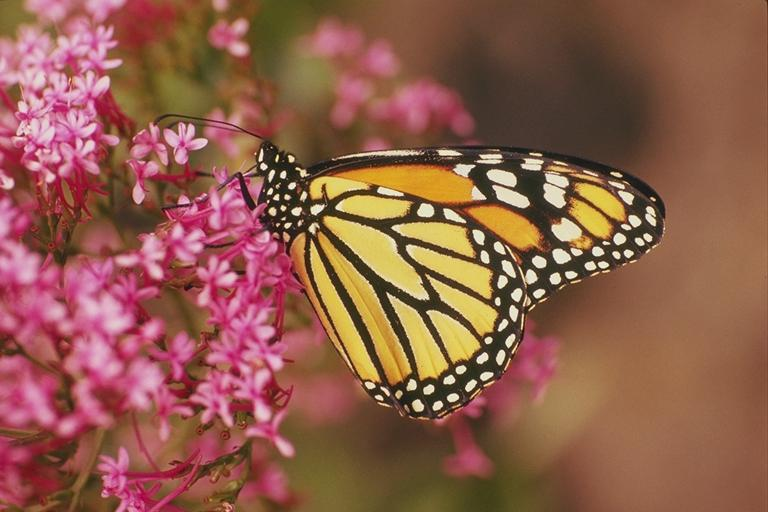
\includegraphics[width=\textwidth]{monarch.jpg}
		\caption{}
		\label{fig:nsi_1}
	\end{subfigure}
	\hfill
	\begin{subfigure}{0.24\textwidth}
		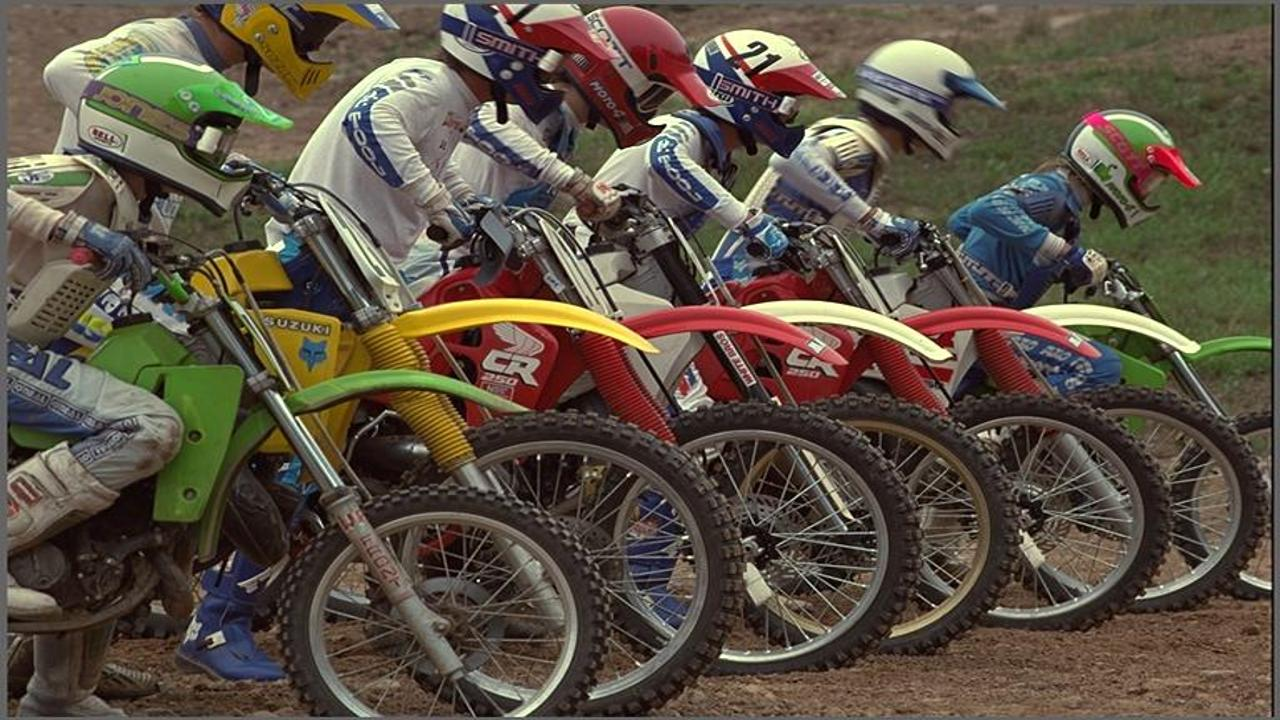
\includegraphics[width=\textwidth]{bikes.jpg}
		\caption{}
		\label{fig:nsi_2}
	\end{subfigure}
	\\
	\begin{subfigure}{0.24\textwidth}
		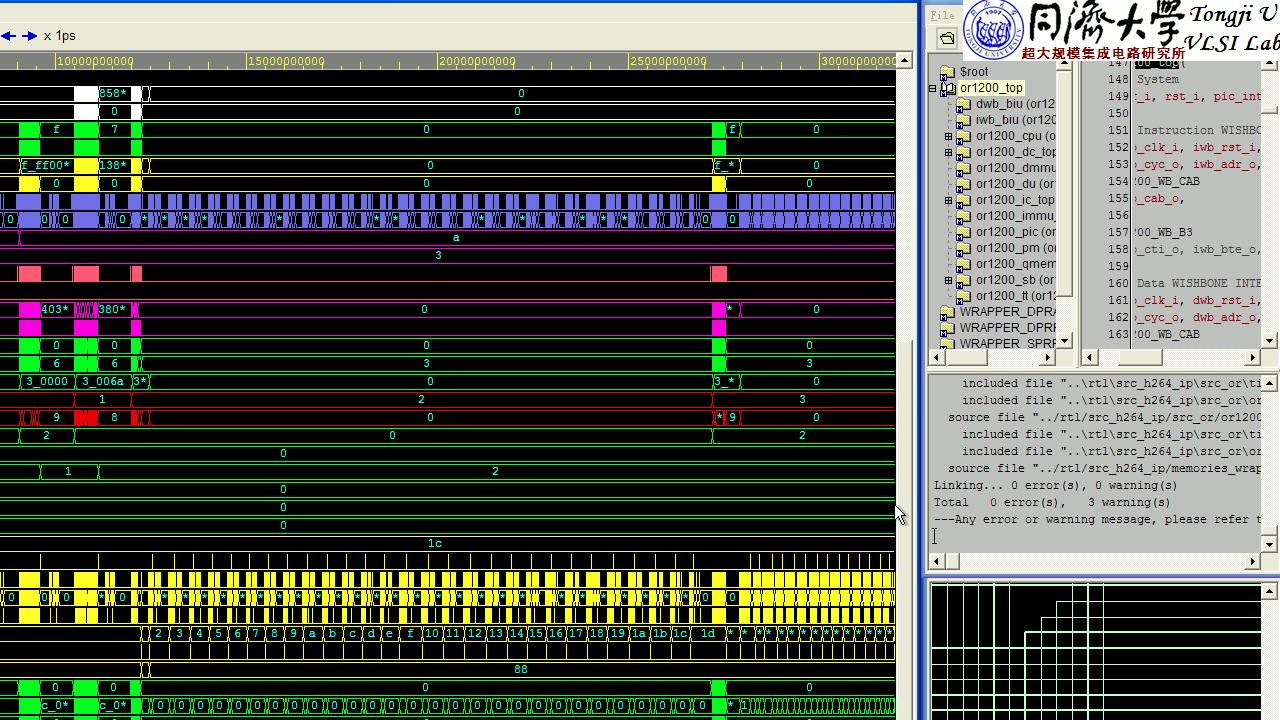
\includegraphics[width=\textwidth]{SCI30.jpg}
		\caption{}
		\label{fig:sci_1}
	\end{subfigure}
	\hfill
	\begin{subfigure}{0.24\textwidth}
		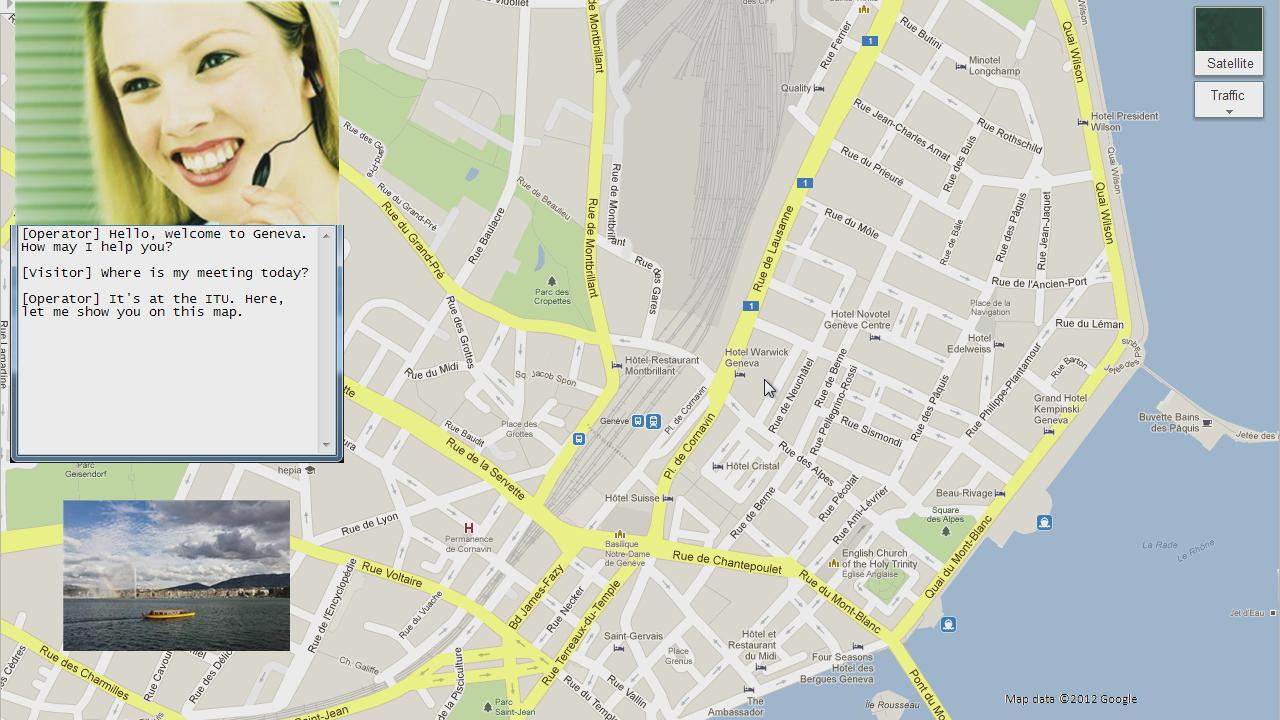
\includegraphics[width=\textwidth]{SCI33.jpg}
		\caption{}
		\label{fig:sci_2}
	\end{subfigure}
	\caption{دو نمونه تصویر طبیعی (در (آ) و (ب)) و دو نمونه نمامفاد (در (ج) و (د))}
	\label{fig:nsi_sci}
\end{figure}


در این قسمت، نحوه‌ی آموزش و آزمون روش‌های اَکْتِ مبتنی بر بردار پشتیبان را مرور کردیم. همچنین، دیدیم که اْکْتِ محاسباتی، کاربردهای مختلفی برای انواع تصاویر دیجیتال دارد. در قسمت بعد، برخی جنبه‌های مربوط به یادگیری ماشین در آموزش \lr{SVR}ها را تحلیل می‌نماییم.
\section{آزمایش‌های پیشنهادی و نتایج} \label{sec:experiments}
در این قسمت می‌بینیم که \lr{SVR}های آموزش‌دیده برای اَکْتْ، ممکن است مشکلاتی از نظر تعمیم‌پذیری داشته باشند. ابتدا یک آزمایش تعریف کرده و سپس به تحلیلِ عملکردِ \lr{SVR} می‌پردازیم.
\subsection{آزمایش پیشنهادی} \label{sec:scenario}
گفتیم که نمامفادها از نوشته‌ها، تصاویر طبیعی و نگاشتارها\LTRfootnote{graphics} تشکیل شده‌اند (قسمت~\ref{sec:domains}). یک راه برای ارزیابی کیفیت نمامفادها، تحلیل جداگانه‌ی این نواحی است \cite{Zhang2018}. اگر یک روش، مختصِّ ارزیابی کیفیت تصاویر اسناد داشته باشیم، به نظر می‌رسد که ترکیبِ آن با روشی مختصِّ تصاویر طبیعی، برای ارزیابی کیفیت نمامفاد، شانس داشته باشد.

$LBPSI(.,.)$ \cite{alaei2016document}، یک روش مرجع کامل، برای اَکْتِ اسناد و نوشته‌هاست. به این ترتیب که اگر $x$ و $y$ مثل (\ref{eq:mse}) تعریف شده باشند، خواهیم داشت:
\begin{equation}
	\text{\lr{LBPSI} {\scriptsize (نمره‌ی کیفیت تخمینی به وسیله‌ی \lr{LBPSI})}} = LBPSI(x, y)
	\label{eq:LBPSI}
\end{equation}
همینطور، $SQMS(., .)$ \cite{gu2016saliency}، یک روش مرجع کامل برای نمامفاد است. برای ارزیابی نواحی طبیعی، از $HaarPSI(., .)$ \cite{reisenhofer2018haar} و $GMSD(., .)$ \cite{xue2013gradient} استفاده می‌کنیم که جنبه‌های مختلف ساختاری را می‌سنجند. از آنجایی که ارزیابی تباین\LTRfootnote{contrast} کار دشواری است \cite{shokrollahi2020histogram}، می‌توانیم از $VIF(., .)$ \cite{sheikh2006image} هم استفاده کنیم که در این زمینه دقیق است.

با استفاده از این روش‌ها، می‌توانیم یک روش ترکیبیِ مرجع کامل \cite{okarma2021combined}، برای ارزیابی نمامفادها بسازیم. $\text{SQMS}$، $\text{LBPSI}$، $\text{HaarPSI}$، $\text{GMSD}$ و $\text{VIF}$ را برای $x$ و $y$ محاسبه می‌کنیم. در این صورت، ۵ عدد خواهیم داشت که می‌توانیم با آن‌ها یک بردار ویژگی تشکیل دهیم:
\begin{equation}
	\vec{f} = [\text{SQMS}, \text{LBPSI}, \text{HaarPSI}, \text{GMSD}, \text{VIF}]
	\label{eq:feactor}
\end{equation}
با داشتن این بردار ویژگی، می‌توانیم یک \lr{SVR} را برای نگاشت آن به نمره‌ی کیفیت آموزش دهیم. برای داده‌ی آموزشی، از مجموعه‌داده‌های کیفیت نمامفاد، به نام‌های \lr{SIQAD} \cite{yang2015perceptual} و \lr{SCID} \cite{ni2017} استفاده می‌کنیم.

\lr{SIQAD} شامل ۲۰ تصویر مرجع است، که هر کدام با ۷ نوع تخریب، تغییر یافته‌اند. هر تخریب در ۷ سطح اعمال شده است. بنابراین، $7\times7\times20=980$ تصویر تخریب‌شده در \lr{SIQAD} وجود دارد. علاوه بر تخریب‌های \lr{SIQAD}، \lr{SCID} دو تخریب دیگر را نیز به ۴۰ تصویرِ مرجعِ خود اعمال کرده است. هر تخریب در ۵ سطحِ شدّت شبیه‌سازی شده است، لذا در \lr{SCID}، ۱۸۰۰ تصویر تخریب‌شده موجود است. برای تصاویر تخریب‌شده در این دو مجموعه‌داده، نمرات کیفیت انسانی تهیه شده است.

علاوه بر (\ref{eq:feactor})، می‌توانیم ترکیب‌های دیگری، مثل $\vec{f}\prime = [SQMS, LBPSI, GMSD]$ را در نظر بگیریم. از آنجایی که $SQMS(., .)$، خود یک روش مختصِّ نمامفاد است، تأثیر ترکیب سایر روش‌ها با آن را را بررسی می‌کنیم. به این ترتیب، ترکیباتی که می‌توان امتحان کرد را در جدول~\ref{tbl:combs} خلاصه نموده‌ایم. برای مثال، $\vec{f}_1$، حاصلِ ترکیبِ $SQMS(., .)$ و $HaarPSI(., .)$ است. یعنی: $\vec{f}_1 = [\text{SQMS}, \text{HaarPSI}]$. یا $\vec{f}_6 = [\text{SQMS}, \text{HaarPSI}, \text{VIF}]$. بدیهی است که برای هر یک از بردارهای ویژگیِ $\vec{f}_1$ تا $\vec{f}_{14}$، باید \lr{SVR}ِ مجزّایی آموزش داده شود. در ادامه، عملکرد هر یک از این مدل‌ها بررسی می‌شوند.

\begin{table}
	\caption{ترکیب‌های درنظر گرفته‌شده برای تشکیل بردار ویژگی. وجودِ \checkmark~به معنی استفاده شدنِ نمره‌ی روشِ آن ستون است.}
	\label{tbl:combs}
	\begin{tabular}{c|c|c|c|c|c}
		بردار& \lr{SQMS}&\lr{HaarPSI}&\lr{GMSD}&\lr{VIF}&\lr{LBPSI}\\
		\hline
		\hline
		$\vec{f}_1$&\checkmark&\checkmark&&&\\
		\hline
		$\vec{f}_2$&\checkmark&&\checkmark&&\\
		\hline
		$\vec{f}_3$&\checkmark&&&\checkmark&\\
		\hline
		$\vec{f}_4$&\checkmark&&&&\checkmark\\
		\hline
		$\vec{f}_5$&\checkmark&\checkmark&\checkmark&&\\
		\hline
		$\vec{f}_6$&\checkmark&\checkmark&&\checkmark&\\
		\hline
		$\vec{f}_7$&\checkmark&\checkmark&&&\checkmark\\
		\hline
		$\vec{f}_8$&\checkmark&&\checkmark&\checkmark&\\
		\hline
		$\vec{f}_9$&\checkmark&&\checkmark&&\checkmark\\
		\hline
		$\vec{f}_{10}$&\checkmark&&&\checkmark&\checkmark\\
		\hline
		$\vec{f}_{11}$&\checkmark&\checkmark&\checkmark&\checkmark&\\
		\hline
		$\vec{f}_{12}$&\checkmark&\checkmark&\checkmark&&\checkmark\\
		\hline
		$\vec{f}_{13}$&\checkmark&\checkmark&&\checkmark&\checkmark\\
		\hline
		$\vec{f}_{14}$&\checkmark&&\checkmark&\checkmark&\checkmark\\
		\hline
	\end{tabular}
	
\end{table}
\subsection{موفقیت ترکیبِ روش‌ها، در هر یک از مجموعه‌داده‌ها} \label{sec:per_dataset}
بردارهای $\vec{f}_1$ تا $\vec{f}_{14}$ را برای نمونه‌های \lr{SIQAD} و \lr{SCID} محاسبه کرده، و اعتبارسنجیِ متقابلِ ۱۰۰۰-لایه را برای یک یکِ آن‌ها انجام می‌دهیم. شکل~\ref{fig:res_per_dataset}، بهره‌وریِ عملکردِ مدل‌های ترکیبی، نسبت به استفاده‌ی مستقیم از \lr{SQMS} را نشان می‌دهد. منظور از بهره‌وری، محاسبه‌ی مقدار زیر است:
\begin{equation}
	\text{بهروه‌وری}_{f_i}= |\text{SROCC}_{f_i}|-|\text{SROCC}_{\text{SQMS}}|
	\label{eq:gain}
\end{equation}
که $i\in\{1, \ldots, 14\}$ و $\text{SROCC}_{f_i}$، ضریب همبستگی اِسْپیِرمَنِ محاسبه‌شده برای \lr{SVR}ی است که روی $f_i$ آموزش دیده باشد. همانطور که در قسمت~\ref{sec:datasets} گفته شد، این ضریب همبستگی، بین نمرات الگوریتم و نمرات انسانی محاسبه می‌شود. $\text{SROCC}_{\text{SQMS}}$ هم دقتِ $SQMS(.,.)$ نشان می‌دهد. می‌بینیم که تمام مدل‌ها عملکرد بهتری نسبت به $SQMS(., .)$ داشته‌اند.
\begin{figure}
	\begin{center}
	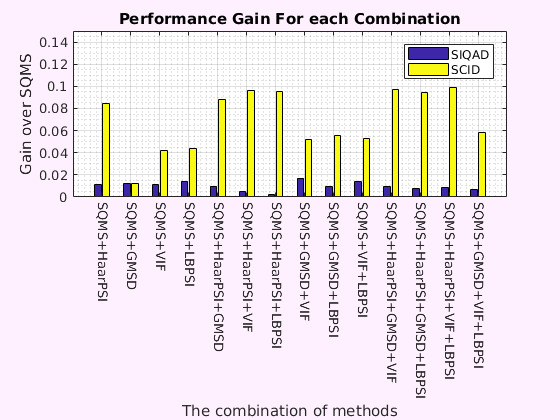
\includegraphics[width=0.47\textwidth]{per_dataset}
	\end{center}
	\caption{بهره‌وری هر یک از روش‌های ترکیبی نسبت به $SQMS(., .)$. برای هر ترکیب، بهره‌وریِ عملکرد بر روی دو محموعه‌داده، با دو رنگ متفاوت نشان داده شده است.}
	\label{fig:res_per_dataset}
\end{figure}
\subsection{عدم تعمیم‌پذیری به تخریب‌های مختلف} \label{sec:gen_dst}
با افزایش دقتِ $SQMS(., .)$، روی کُلِّ مجموعه‌داده، انتظار می‌رود که ترکیب‌ها بهبودی مشابه را روی تک تکِ تخریب‌ها نیز داشته باشند. میزان دقت مدل‌ها روی تخریب‌ها طبق~\ref{sec:perdist} محاسبه گردیده و بهره‌وری آن نسبت به $SQMS(.,.)$ در شکل~\ref{fig:res_per_distortion} نشان داده می‌شود.
\begin{figure*}
	\begin{subfigure}{0.47\textwidth}
		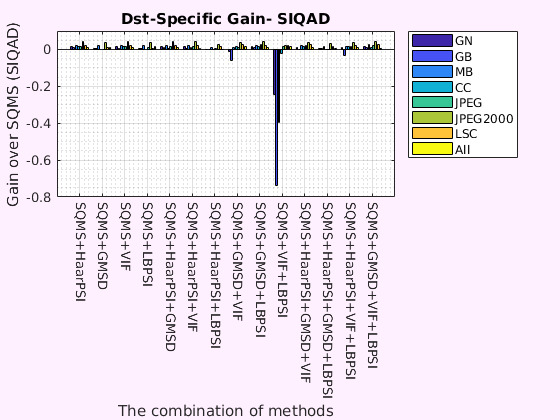
\includegraphics[width=\textwidth]{per_distortion_SIQAD}
		\caption{}
		\label{fig:res_per_distortion_SIQAD}
	\end{subfigure} 
	\hfill
	\begin{subfigure}{0.47\textwidth}
		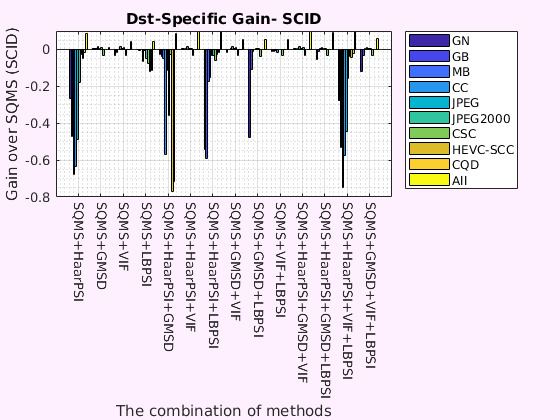
\includegraphics[width=\textwidth]{per_distortion_SCID}
		\caption{}
		\label{fig:res_per_distortion_SCID}
	\end{subfigure}
	\caption{نتیجه‌ی ارزیابی به ازای هر تخریب. نتایج \lr{SIQAD} در (آ) و \lr{SCID} در (ب) قابل ملاحظه هستند. بهره‌وری به ازای هر تخریب، با رنگ متفاوتی مشخص شده است.}
	\label{fig:res_per_distortion}
\end{figure*}
می‌بینیم که نه تنها همه‌ی مدل‌ها عملکرد مشابهی نداشتند، بلکه در بسیاری از موارد، بهره‌وری منفی بوده است. کاملاً منطقی است که یکی از علّت‌ها را ضعف بردارهای ویژگی بدانیم. فارغ از این نظریه، مسئله‌ی دیگری وجود دارد که باید در نظر گرفته شود و آن \emph{فراعامل‌ها} هستند. 

همانطور که در انتهای~\ref{sec:trainSVR} گفته شد، بهینه‌سازیِ $c$ و $\gamma$ با اعتبارسنجیِ متقابلِ ۱۰۰-لایه صورت می‌گیرد:
\begin{equation}
	\begin{aligned}
	(c^*, \gamma ^*) = \\
		\text{opt}(r_c, r_\gamma, \text{dataset}_{80, \text{all}}, \text{dataset}_{20, \text{all}}, 100)
	\end{aligned}
	\label{eq:cazama}
\end{equation}
رابطه‌ی~\ref{eq:cazama} مواردی که باید در نظر گرفته شوند را خلاصه می‌کند. $c^*$ و $\gamma^*$ فراعامل‌های بهینه هستند. تابع $\text{opt}$ نتایج بهینه‌سازی را برمی‌گرداند. $r_c$ و $r_\gamma$، به ترتیب، مجموعه‌ی مقادیری هستند که برای $c$ و $\gamma$ امتحان می‌شوند. مثلاً اگر $r_c = \{1, 10, 10^2, 10^3, 10^4, 10^5, 10^6\}$ باشد، بهترین مقدار برای $c$ از این مجموعه پیدا می‌شود. مقادیر مورد بررسی به صورت دستی انتخاب شده و تعدادشان به توان پردازشی در دسترس بستگی دارد. در هر بار آموزش و ارزیابی، نیاز به یک مجموعه‌ی آموزش و یک مجموعه‌ی آزمون داریم.

طبق رابطه‌ی\ref{eq:cazama}، مجموعه‌ی آموزش، $\text{dataset}_{80, \text{all}}$ است. این عبارت یک زیرمجموعه از نمونه‌های مجموعه‌داده‌ی $\text{dataset}$ را مشخص می‌نماید. این زیرمجموعه، عبارت است از \textbf{همه}ی ($\text{all}$) تخریب‌های موجود در زیرمجموعه‌ی آموزشِ افرازِ ۸۰-۲۰. برخی نمونه‌ها از این عبارت، می‌توانند $\text{SIQAD}_{80, \text{JPEG}}$ و $\text{SCID}_{20, \text{GB}}$ باشند. که اوّلی، یعنی تمامیِ نمونه‌های \lr{SIQAD}؛ که در افرازِ ۸۰-۲۰، در مجموعه‌ی آموزش قرار گرفته‌اند؛ و تخریبِ آن‌ها از نوعِ $\text{JPEG}$ است. دومی، نمونه‌هایی از \lr{SCID} را مشخص می‌کند که در مجموعه‌ی آزمون قرار گرفته‌اند و تخریبِ آن‌ها از نوعِ $\text{GB}$\RTLfootnote{نوعی تار شدگی تصویر. برای شرح سایر تخریب‌ها به مقاله‌ی خودِ مجموعه‌داده‌ها رجوع شود.} است. آخرین ورودیِ تابعِ $\text{opt}$ هم، تعداد لایه‌های (دفعاتِ) اعتبارسنجیِ متقابل است.

اگر به جای $\text{opt}(r_c, r_\gamma, \text{SIQAD}_{80, all}, \text{SIQAD}_{20, all}, 100)$، از $\text{opt}(r_c, r_\gamma, \text{SIQAD}_{80, all}, \text{SIQAD}_{20, \text{JPEG}}, 100)$ استفاده کنیم، نتایج متفاوت خواهند بود (شکل~\ref{fig:res_per_dist_hyper}). قبل از بررسیِ نتایج، یک رابطه مانند~\ref{eq:cazama} برای اعتبارسنجیِ متقابل قرارداد می‌کنیم، که نقشِ فراعامل‌ها را نیز در نظر بگیرد:
\begin{equation}
	\begin{aligned}
	\text{دقّت الگوریتم} = \\
		\displaystyle cv(\text{dataset}_{80, \text{all}}, \\
		\text{opt}(r_c, r_\gamma, \text{dataset}_{80, \text{all}}, \text{dataset}_{20, \text{all}}, 100),\\
		\text{dataset}_{20, \text{all}}, 1000)
	\end{aligned}
	\label{eq:parama}
\end{equation}
تابعِ $cv(.,.,.,.)$، چهار  ورودی دارد که عبارت‌اند از: مجموعه‌ی آموزش، فراعامل‌های بهینه، مجموعه‌ی آزمون و تعداد لایه‌های اعتبارسنجیِ متقابل. این تابع میانه‌ی $\text{SROCC}$های محاسبه‌شده در ۱۰۰۰ مرتبه را بر می‌گرداند.
\begin{figure*}
	\begin{subfigure}{0.47\textwidth}
		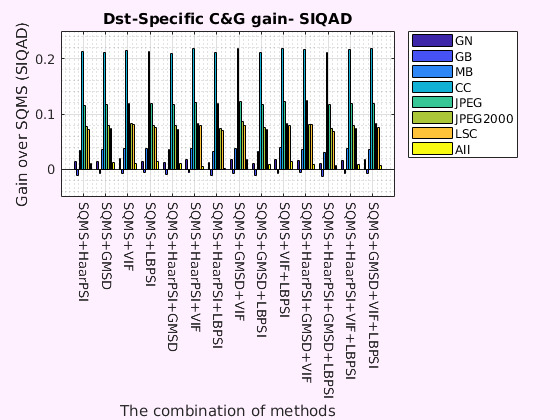
\includegraphics[width=\textwidth]{per_distortion_hyper_SIQAD}
		\caption{}
		\label{fig:res_per_distortion_SIQAD_hyper}
	\end{subfigure} 
	\hfill
	\begin{subfigure}{0.47\textwidth}
		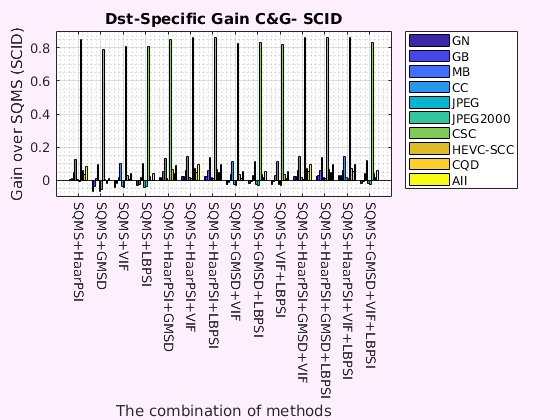
\includegraphics[width=\textwidth]{per_distortion_hyper_SCID}
		\caption{}
		\label{fig:res_per_distortion_SCID_hyper}
	\end{subfigure}
	\caption{نتیجه‌ی ارزیابی به ازای هر تخریب بعد از بهینه‌سازی فراعامل‌ها روی هر یک از تخریب‌ها. نتایج \lr{SIQAD} در (آ) و \lr{SCID} در (ب) قابل ملاحظه هستند.}
	\label{fig:res_per_dist_hyper}
\end{figure*}

شکل~\ref{fig:res_per_dataset} نتایج را برای آزمایش زیر نشان می‌دهد:
\begin{equation}
	\begin{aligned}
		\displaystyle cv(\text{dataset}_{80, \text{all}}, \\
		\text{opt}(r_c, r_\gamma, \text{dataset}_{80, \text{all}}, \text{dataset}_{20, \text{all}}, 100),\\
		\text{dataset}_{20, \text{all}}, 1000)
	\end{aligned}
	\label{eq:per_dataset}
\end{equation}
که $\text{dataset}$ در هر بار، یا $\text{SIQAD}$ و یا $\text{SCID}$ است. برای ارزیابی روی هر یک از تخریب‌ها (شکل~\ref{fig:res_per_distortion})، رابطه (\ref{eq:per_dataset}) به شکل زیر تغییر می‌کند:
\begin{equation}
	\begin{aligned}
		\displaystyle cv(\text{dataset}_{80, \text{all}}, \\
		\text{opt}(r_c, r_\gamma, \text{dataset}_{80, \text{all}}, \text{dataset}_{20, \text{all}}, 100),\\
		\text{dataset}_{20, \text{dst}}, 1000)
	\end{aligned}
	\label{eq:per_distortion}
\end{equation}
که $\text{dataset}$ مطابقِ (\ref{eq:per_dataset}) و $\text{dst}\in \{\text{تخریب‌های موجود در \lr{dataset}}\}$.
اگر در آزمایشی که رابطه (\ref{eq:per_distortion}) نشان می‌دهد، فراعامل‌ها را روی تخریب‌های متناظر بهینه کنیم، نتایجِ شکل~\ref{fig:res_per_dist_hyper} حاصل می‌شوند. به طور رسمی، نتایج شکل~\ref{fig:res_per_dist_hyper}، حاصلِ آزمایشِ زیر هستند:
\begin{equation}
	\begin{aligned}
		\displaystyle cv(\text{dataset}_{80, \text{all}}, \\
		\text{opt}(r_c, r_\gamma, \text{dataset}_{80, \text{all}}, \text{dataset}_{20, \text{dst}}, 100),\\
		\text{dataset}_{20, \text{dst}}, 1000)
	\end{aligned}
	\label{eq:per_dist_hyper}
\end{equation}
پس می‌بینیم که علاوه بر تأثیرِ احتمالیِ بردارهای ویژگی، فراعامل‌ها نیز نقش مهمی در عملکرد \lr{SVR}ها دارند.
\subsection{عدم تعمیم‌پذیری به سایر مجموعه‌داده‌ها} \label{sec:gen_cross}
برای بررسی عدمِ وابستگیِ یک مدل به صحنه‌های یک مجموعه‌داده، آن را روی یک مجموعه‌داده آموزش داده و روی مجموعه‌داده‌ی دیگر می‌آزمایند: 
\begin{equation} 
	\begin{aligned} 
		\displaystyle cv(\text{SIQAD}_{\text{all}, \text{all}}, \\
		\text{opt}(r_c, r_\gamma, \text{SIQAD}_{80, \text{all}}, \text{SIQAD}_{20, \text{all}}, 100),\\
		\text{SCID}_{\text{all}, \text{all}}, 1)
	\end{aligned}
	\label{eq:siqad_scid}
\end{equation}
\begin{equation} 
	\begin{aligned} 
		\displaystyle cv(\text{SCID}_{\text{all}, \text{all}}, \\
		\text{opt}(r_c, r_\gamma, \text{SCID}_{80, \text{all}}, \text{SCID}_{20, \text{all}}, 100),\\
		\text{SIQAD}_{\text{all}, \text{all}}, 1)
	\end{aligned}
	\label{eq:scid_siqad}
\end{equation}
شکل~\ref{fig:cross_dataset} نتایج را برای آزمایش‌های (\ref{eq:scid_siqad}) و (\ref{eq:siqad_scid}) نشان می‌دهد.

\begin{figure}
	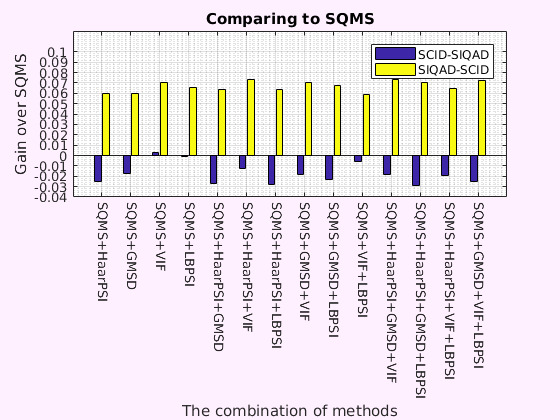
\includegraphics[width=0.47\textwidth]{cross_whole.jpg}
	\caption{نتایج آزمونِ تعمیم‌پذیری. ستون‌های زرد مربوط به آموزش روی \lr{SIQAD} و آزمون روی \lr{SCID} هستند. ستون‌های سُرمه‌ای مربوط به آموزش و آزمونِ عکس هستند.}
	\label{fig:cross_dataset}
\end{figure}
می‌بینیم که بهبودِ مشاهده شده در آزمایش (\ref{eq:per_dataset}) (با نتایجِ قابلِ مشاهده در شکل~\ref{fig:res_per_dataset}) برای \lr{SIQAD} اتفاق نمی‌افتد. به غیر از این مسئله، اگر مدلِ آموزش‌دیده را برای تک تکِ تخریب‌ها بیازمائیم، باز هم با اُفْتِ عملکردی مشابهِ قسمتِ\ref{sec:gen_dst} مشابه می‌شویم. بیان رسمیِ این آزمایش‌ها در روابط (\ref{eq:scid_siqad_dst}) و (\ref{eq:siqad_scid_dst}) و نتایج آن‌ها در شکل~\ref{fig:cross_dst} ارائه شده‌اند.
\begin{equation} 
	\begin{aligned} 
		\displaystyle cv(\text{SCID}_{\text{all}, \text{dst}}, \\
		\text{opt}(r_c, r_\gamma, \text{SCID}_{80, \text{all}}, \text{SCID}_{20, \text{all}}, 100),\\
		\text{SIQAD}_{\text{all}, \text{dst}}, 1)
	\end{aligned}
	\label{eq:scid_siqad_dst}
\end{equation}
\begin{equation} 
	\begin{aligned} 
		\displaystyle cv(\text{SIQAD}_{\text{all}, \text{dst}}, \\
		\text{opt}(r_c, r_\gamma, \text{SIQAD}_{80, \text{all}}, \text{SIQAD}_{20, \text{all}}, 100),\\
		\text{SCID}_{\text{all}, \text{dst}}, 1)
	\end{aligned}
	\label{eq:siqad_scid_dst}
\end{equation}
$\text{dst}$ در روابط بالا، عضوِ مجموعه‌ی تخریب‌هایی است که در \lr{SCID} و \lr{SIQAD} مشترک هستند. می‌بینیم که نتایج بهترِ آزمون تعمیم‌پذیری برای مجموعه‌ی \lr{SCID} هم به تک تکِ تخریب‌های آن قابل تعمیم نیست.
\begin{figure*}
	\begin{subfigure}{0.47\textwidth}
		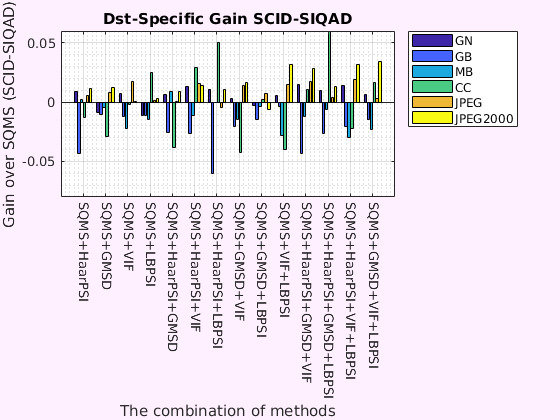
\includegraphics[width=\textwidth]{cross_SCID_SIQAD_dst}
		\caption{}
		\label{fig:scid_siqad_dst}
	\end{subfigure} 
	\hfill
	\begin{subfigure}{0.47\textwidth}
		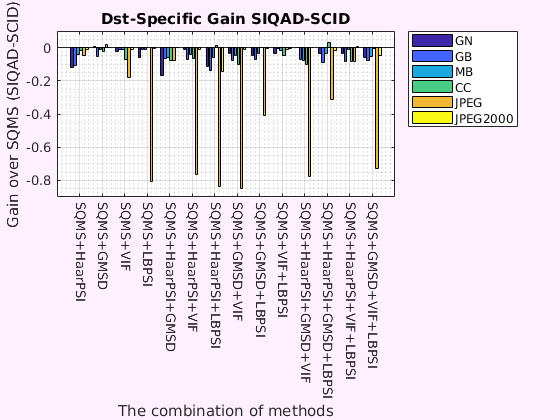
\includegraphics[width=\textwidth]{cross_SIQAD_SCID_dst}
		\caption{}
		\label{fig:siqad_scid_dst}
	\end{subfigure}
	\caption{نتایجِ ارزیابی هر تخریب، وقتی مجموعه‌داده‌های آموزش و آزمون متفاوت‌اند. (آ): برای $\text{SCID}\rightarrow \text{SIQAD}$ و (ب) برای $\text{SIQAD}\rightarrow \text{SCID}$}
	\label{fig:cross_dst}
\end{figure*}
\section{جمع‌بندی} \label{sec:conclusion}
در این مقاله بردارهای پشتیبان را، طبق روش رایج، برای اَکْتْ آموزش دادیم. دیدیم که وقتی گزارش عملکرد به روش رایج انجام می‌شود، نقش فراعامل‌ها هم باید بازتاب گردد. یک فرمول‌بندی ارائه شد که این موارد را لحاظ نماید. تأثیرِ بهینه‌سازیِ فراعامل‌ها را مشاهده کردیم و دیدیم که به این مسئله در آزمایش‌های ارزیابی کیفیت پرداخته نمی‌شود. محدود بودنِ تصاویر مجموعه‌داده‌ها، نگرانی در موردِ تعمیم‌پذیری مدل‌ها به تصاویر دنیای واقعی را بیشتر می‌کند. مخصوصاً وقتی که تخریب‌های مجموعه‌داده‌ها مصنوعی بوده و ممکن است با تخریب‌های طبیعی متفاوت باشند. شاید بهتر باشد که نحوه‌ی بهینه‌سازیِ فراعامل‌های مدل‌های یادگیری نیز در گزارش‌های عملکرد مقالات تشریح گردد. آزمایش‌های انجام‌شده با کُدهای موجود در \href{https://github.com/cheraaqee/fusion\_iqa}{https://github.com/cheraaqee/fusion\_iqa} قابلِ شبیه‌سازی هستند.
\bibliographystyle{ieeetr-fa}
\bibliography{ref}
\end{document}
